\begin{center}
  \vspace{1em}
  \textbf{\Large Largest Concatenation-Component in Regular Expressions}
  \vspace{1em}
\end{center}

Hyperscan implements algorithms to decompose regexes into literals and FA in its Rose engine. There may be a relation between how well a regex can be decomposed and the size of its largest concatenation-component.

\section{Recurrences}

Let $\A$ be a finite alphabet and $\T$ be the set of all regexes excluding $\epsilon$ over $\A$. The size function $|\cdot|$ is the number of nodes.

\begin{definition}[BST-like distribution for regexes]
  We define $p:\T \to [0,1]$ as follows.
  \begin{enumerate}
    \item $\sum\limits_{c\in\A}p(c) = 1$,
    \item $p\left(\vcenter{\hbox{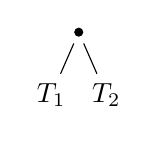
\begin{tikzpicture}[level distance=8mm, sibling distance=7mm, edge from parent/.style={draw, shorten <=1mm}]
                  \node[circle, draw, fill=black, minimum size=1mm, inner sep=0pt] {}
                  child { node {$T_1$} }
                  child { node {$T_2$} };
                \end{tikzpicture}}}\right) = \dfrac{u}{n-2} p(T_1)p(T_2)$, where $|T_1| + |T_2| = n-1$.
    \item $p\left(\vcenter{\hbox{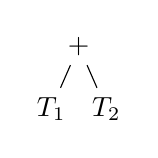
\begin{tikzpicture}[level distance=8mm, sibling distance=7mm]
                  \node{$+$}
                  child { node {$T_1$} }
                  child { node {$T_2$} };
                \end{tikzpicture}}}\right) = \dfrac{v}{n-2} p(T_1)p(T_2)$, where $|T_1| + |T_2| = n-1$.
    \item $p\left(\vcenter{\hbox{\begin{tikzpicture}[level distance=8mm, sibling distance=7mm]
                  \node{$*$}
                  child { node {$T$} };
                \end{tikzpicture}}}\right) = (1-u-v) p(T)$.
  \end{enumerate}
\end{definition}

We want to compute the expected size of the largest all-concatenation component in a regex over all of equivalent forms of its parse tree. The reason is as follows. Take the regex
$$(abc + d)(xy+z) = abcxy + abcxz + dxy + dz.$$
We expect the largest concatenation-component to be in $abcxy$ instead of $abc$ because the former is extracted by Hyperscan. Therefore, a subtree may \textit{yield} its concatenation-component to its parent if the parent is a concatenation node.

Recall the construction
$$\T = \sum_{c \in \A} c + \vcenter{\hbox{\begin{tikzpicture}[level distance=8mm, sibling distance=7mm]
        \node{$*$}
        child { node {$\T$} };
      \end{tikzpicture}}} + \vcenter{\hbox{\begin{tikzpicture}[level distance=8mm, sibling distance=7mm, edge from parent/.style={draw, shorten <=1mm}]
        \node[circle, draw, fill=black, minimum size=1mm, inner sep=0pt] {}
        child { node {$\T$} }
        child { node {$\T$} };
      \end{tikzpicture}}} + \vcenter{\hbox{\begin{tikzpicture}[level distance=8mm, sibling distance=7mm]
        \node{$+$}
        child { node {$\T$} }
        child { node {$\T$} };
      \end{tikzpicture}}}.$$
Define the random variables
\begin{enumerate}
  \item $M_n$: the largest concatenation-component that is not inside a Kleene star of a regex of size $n$ \textit{itself},
  \item $Y_n$: the largest concatenation-component that is not inside a Kleene star of a regex of size $n$ that it \textit{yields} to its parent.
\end{enumerate}

We have the following recurrences
\begin{align}
  Y_{n+2}
   & =\begin{cases}
        Y_{U_n}^{(1)} + Y_{n+1-U_n}^{(2)} + 1  & \text{prob. } u,    \\
        \max(Y_{U_n}^{(1)}, Y_{n+1-U_n}^{(2)}) & \text{prob. } v,    \\
        0                                      & \text{prob. } 1-u-v
      \end{cases}                                                                      & Y_1=Y_2=0.                         \label{eq:yield}                           \\
  M_{n+2}
   & = \begin{cases}
         \max(Y_{U_n}^{(1)} + Y_{n+1-U_n}^{(2)} + 1, M_{U_n}^{(1)}, M_{n+1-U_n}^{(2)}) & \text{prob. } u,    \\
         \max(M_{U_n}^{(1)}, M_{n+1-U_n}^{(2)})                                        & \text{prob. } v     \\
         0                                                                             & \text{prob. } 1-u-v
       \end{cases} & M_1=M_2=0.
\end{align}

We have used $Y_n^{(1)}, Y_n^{(2)}, M_n^{(1)}, M_n^{(2)}$ as independent copies of $Y_n$ and $M_n$ respectively, and $U_n$ as a uniform random variable over $\{1, 2, \ldots, n\}$ independent of all $Y_n^{(i)}$ and $M_n^{(i)}$.

\section{The yield recurrence}

\subsection{Lower and upper bounds}

We rewrite the recurrence (\ref{eq:yield}) as
\begin{equation}
  Y_{n+2} \stackrel{d}{=} I\left(Y_{U_n}^{(1)} + Y_{n+1-U_n}^{(2)} + 1\right) + J\max\left(Y_{U_n}^{(1)}, Y_{n+1-U_n}^{(2)}\right), \label{eq:yield_indicator}
\end{equation}

where $I$ and $J$ are independent Bernoulli random variables taking value $1$ with probability $u$ and $v$ respectively such that $I+J\le 1$, and $Y_n^{(1)}, Y_n^{(2)}$ are independent copies of $Y_n$. The notion of equality is in distribution. Note that we can reuse the same $Y_n^{(1)}, Y_n^{(2)}$ and $U_n$ for the second term because the two terms are mutually exclusive.

Let $y_n=\EE[Y_n]$. Take expectation on both sides, we have
$$y_{n+2} = u + \dfrac{2u}{n}\sum_{i=1}^{n}y_i + \dfrac{v}{n}\sum_{i=1}^{n}\EE[\max(Y_i, Y_{n+1-i})].$$

For the upper bound, we use the fact that $\max(Y_i, Y_{n+1-i}) \le Y_i + Y_{n+1-i}$, which gives an upper bound sequence
\begin{equation}
  y_{n+2}^U = u + \dfrac{2(u+v)}{n}\sum_{i=1}^{n}y_i^U, \quad y_1^U=y_2^U=0.
  \label{eq:upper_bound}
\end{equation}

For the lower bound, we use
\begin{align*}
  \EE[\max(Y_i, Y_{n+1-i})]
   & = \EE\left[\dfrac{1}{2}(Y_i + Y_{n+1-i} + |Y_i - Y_{n+1-i}|)\right]                   \\
   & \ge \dfrac{1}{2}(\EE[Y_i] + \EE[Y_{n+1-i}]) + \dfrac{1}{2}|\EE[Y_i] - \EE[Y_{n+1-i}]| \\
   & = \dfrac{1}{2}(y_i + y_{n+1-i} + |y_i - y_{n+1-i}|).
\end{align*}

This gives the lower bound sequence
\begin{equation}
  \label{eq:lower_bound}
  y_{n+2}^L = u + \dfrac{2u+v}{n}\sum_{i=1}^{n}y_i^L + \dfrac{v}{n}\sum_{i=1}^{n}|y_i^L - y_{n+1-i}^L|, \quad y_1^L=y_2^L=0.
\end{equation}

\begin{remark}
  Another lower bound is obtained by Jensen's inequality as follows.
  $$\EE[\max(Y_i, Y_{n+1-i})] \ge \max(\EE[Y_i], \EE[Y_{n+1-i}]) = \max(y_i, y_{n+1-i}) = y_{\max(i, n+1-i)},$$
  where the last equality holds because $y_n$ is non-decreasing in $n$. This gives the following lower bound sequence
  \begin{align}
    y_{n+2}^{L'} & = u + \dfrac{2u}{n}\sum_{i=1}^{n}y_i^{L'} + \dfrac{2v}{n}\sum_{i=\lfloor (n+1)/2 \rfloor}^{n}y_{i}^{L'}, & y_1^{L'}=y_2^{L'}=0.
  \end{align}
\end{remark}

Looking at the bounds (\ref{eq:lower_bound}) and (\ref{eq:upper_bound}), there are four regimes that are worth considering
\begin{enumerate}
  \item If $2u+v>1$, the bounds are polynomials. This case agrees well with the empirical data.
  \item $2(u+v) = 1$.
  \item $2u+v=1$.
  \item $2(u+v)<1$.
\end{enumerate}


\subsection{Asymptotic when both bounds are polynomial}

Consider the case $2u+v>1$. By the bounds,  there exists
$$\alpha = \inf\left\{\beta: \dfrac{Y_n}{n^\beta} \xlongrightarrow{d} 0\right\}.$$

We know that $\alpha \in (2u+v-1, 2(u+v)-1]$. We want to see if indeed $y_n \sim C n^\alpha$ for some $C>0$.

We try the contraction method \cite{ludgercontraction,neininger2004general, drmota2009random}. Let us mention some conventions. For a random variable $X$, denote by $\L(X)$ its distribution. Let $(\M, d)$ be a metric space where $\M$ is a set of probability distributions of our random variables and the metric $d$ is such that $d(\L(X),\L(Y))=0$ implies $X \stackrel{d}{=} Y$. The idea is as follows

\begin{enumerate}
  \item Guess a normalization $X_n$ of $Y_n$ that converges in distribution.
  \item Plug $X_n$ into the recurrence. Assume that $X_n$ converges, show that the limit equation has a unique solution $X^*$. This is done by proving that the operator $T$ defined by the right-hand side of the limit equation is a contraction.
  \item Prove that indeed $d(\L(X_n), \L(X^*)) \to 0$.
\end{enumerate}

The method is use to obtain more information about the limit distribution of $X_n$ rather than just its expectation. For example, the following is the recurrence for the number of comparisons in Quicksort where the first element is chosen as the pivot \cite{drmota2009random}
$$Y_{n} = Y_{U_n}^{(1)} + Y_{n-1-U_n}^{(2)} + n-1.$$
One can find the asymptotic of $\EE[Y_n]$ by taking expectation on both sides. The contraction is then used to show that $X_n = \dfrac{Y_n - \EE[Y_n]}{n}\to X^*$, where the denominator $n$ is the ``guessed'' variance.

Our case is weaker. The normalization is $X_n = Y_n / n^{\alpha}$ such that $X_n\xlongrightarrow{d}X^*$. Plugging into the recurrence (\ref{eq:yield_indicator}), we have
\begin{align*}
  (n+2)^\alpha X_{n+2} \stackrel{d}{=} \,\,
   & I\left(U_n^\alpha X_{U_n}^{(1)} + (n+1-U_n)^\alpha X_{n+1-U_n}^{(2)} + 1\right)  \\
   & + J\max\left(U_n^\alpha X_{U_n}^{(1)}, (n+1-U_n)^\alpha X_{n+1-U_n}^{(2)}\right)
\end{align*}
Equivalently,
\begin{equation}
  \begin{aligned}
    X_{n+2} \stackrel{d}{=}\,\,
     & I\left(\left(\dfrac{U_n}{n+2}\right)^\alpha X_{U_n}^{(1)} + \left(\dfrac{n+1-U_n}{n+2}\right)^\alpha X_{n+1-U_n}^{(2)} + \dfrac{1}{(n+2)^\alpha}\right) \\
     & + J\max\left(\left(\dfrac{U_n}{n+2}\right)^\alpha X_{U_n}^{(1)}, \left(\dfrac{n+1-U_n}{n+2}\right)^\alpha X_{n+1-U_n}^{(2)}\right)
  \end{aligned}
\end{equation}

\begin{proposition}
  The right-hand side of the above recurrence converges in distribution to
  \begin{equation}
    I\left(U^\alpha X^{(1)} + (1-U)^\alpha X^{(2)}\right) + J\max\left(U^\alpha X^{(1)}, (1-U)^\alpha X^{(2)}\right)
  \end{equation}
\end{proposition}

\begin{lemma}
  Let $U_n$ be a uniform random variable on $\{1, 2, \ldots, n\}$ and let $U$ be a uniform random variable on $[0,1]$. Then $\dfrac{U_n}{n}\xlongrightarrow{d} U$.
\end{lemma}

\begin{proof}
  Recall that the CFD of $U$ is
  $$F_U(x) = \begin{cases}
      0 & x < 0,         \\
      x & 0 \le x \le 1, \\
      1 & x > 1.
    \end{cases}$$
  Let $V_n = U_n/n$. We have $F_{V_n}(x) = \PP(U_n/n \le x) = \PP(U_n\le nx)$. Hence
  \begin{itemize}
    \item If $x\le 0$, then $F_{V_n}(x) = 0 = F_U(x)$, since $U_n\ge 1$.
    \item If $x > 1$, then $F_{V_n}(x) = 1 = F_U(x)$, since $U_n\le n$.
    \item If $0 < x \le 1$, then $F_{V_n}(x) = \dfrac{\lfloor nx \rfloor}{n}$. Since $x - \dfrac{1}{n} \le \dfrac{\lfloor nx \rfloor}{n} \le x$, we have $F_{V_n}(x) \to x = F_U(x)$.
  \end{itemize}
\end{proof}

Back to our case. By Slutsky's theorem, we have $\dfrac{U_n}{n+2} = \dfrac{U_n}{n} \cdot \dfrac{n}{n+2} \xlongrightarrow{d} U$ as $n \to \infty$. Similarly, we have $\dfrac{n+1-U_n}{n+2} \xlongrightarrow{d} 1-U$.

\begin{lemma}
  Let $(X_n)$ be a sequence of random variables converging in distribution to $X$. Let $(N_n)$ be a integer-valued sequence of random variables independent of $(X_n)$ such that $N_n \xlongrightarrow{d} \infty$. Then $X_{N_n} \xlongrightarrow{d} X$.
\end{lemma}

\begin{proof}
  We want to show that $\lim\limits_{n \to \infty} \PP(X_{N_n} \le x) = \PP(X \le x)$ for all $x$ at which $F_X$ is continuous. The CDF of $X_{N_n}$ is
  $$\PP(X_{N_n} \le x) = \sum_{k=1}^\infty \PP(X_k \le x, N_n = k) = \sum_{k=1}^\infty\PP(N_n = k)\PP(X_k\le k),$$
  where the last equality holds because $X_k$ and $N_n$ are independent. Let $\epsilon > 0$. Since $X_n \xlongrightarrow{d} X$, there exists $K$ such that for all $k\ge K$, we have
  $$|\PP(X_k \le x) - \PP(X \le x)| < \dfrac{\epsilon}{2}.$$
  Since $\sum\limits_{k=1}^\infty\PP(N_n = k) = 1$, we have
  \begin{align*}
    \left|\PP(X_{N_n} \le x) - \PP(X \le x)\right|
     & = \left|\sum_{k=1}^\infty\PP(N_n = k)\left(\PP(X_k\le k) - \PP(X \le x)\right)\right|               \\
     & \le \sum_{k=1}^\infty\PP(N_n = k)\left|\PP(X_k\le k) - \PP(X \le x)\right|                          \\
     & \le \sum_{k=1}^{K-1}\PP(N_n = k)\left|\PP(X_k\le k) - \PP(X \le x)\right|                           \\
     & \,\,\,\, +  \sum_{k=K}^\infty\PP(N_n = k)\left|\PP(X_k\le k) - \PP(X \le x)\right|                  \\
     & \le \sum_{k=1}^{K-1}\PP(N_n = k) \cdot 1 +  \sum_{k=K}^\infty\PP(N_n = k) \cdot \dfrac{\epsilon}{2} \\
  \end{align*}
  Since $N_n \xlongrightarrow{d} \infty$, we have $\PP(N_n \ge K) \to 1$ as $n \to \infty$. Hence, there exists $N$ such that for all $n\ge N$, we have $\PP(N_n \ge K) > 1 - \dfrac{\epsilon}{2}$. Therefore, for all $n\ge N$, we have
  $$\left|\PP(X_{N_n} \le x) - \PP(X \le x)\right| < \dfrac{\epsilon}{2} + \dfrac{\epsilon}{2}\left(1- \dfrac{\epsilon}{2}\right) \le \epsilon.$$

  Since $\epsilon$ is arbitrary, the result follows.
\end{proof}

We want to show that
$$\left(\dfrac{U_n}{n+2}\right)^\alpha X_{U_n}^{(1)} + U^\alpha X^{(1)} + \left(\dfrac{n+1-U_n}{n+2}\right)^\alpha X_{n+1-U_n}^{(2)} \xlongrightarrow{d} U^\alpha X^{(1)} + (1-U)^\alpha X^{(2)}.$$

We already have the function $(u,v,x,y)\mapsto u^\alpha x + v^\alpha y$ being continuous. In order to use the Continuous Mapping Theorem, we need to show that the joint distribution of

$$\left(\dfrac{U_n}{n+2}, \dfrac{n+1-U_n}{n+2}, \dfrac{X_{U_n}^{(1)}}{n+2}, \dfrac{X_{n+1-U_n}^{(2)}}{n+2}\right)$$

converges.

\begin{proposition}
  Let $T:\M_1\to \M_1$ be an operator in the space of probability distributions with finite first moment, defined by

  $$T(\mu) = \L\left(I(U^\alpha X^{(1)} + (1-U)^\alpha X^{(2)}) + J\max(U^\alpha X^{(1)}, (1-U)^\alpha X^{(2)})\right),$$
  where $X^{(1)}, X^{(2)} \overset{\text{iid}}{\sim} \mu$ and $U, I, J$ are independent of $X^{(1)}, X^{(2)}$, defined as in (\ref{eq:yield_indicator}).

  Then $T$ is a contraction in the $(\M_1, \ell_1)$ space, where the $\ell_1$ metric is defined by
  $$\ell_1(\mu, \nu) = \inf\{\EE[|X-Y|]: X\sim \mu, Y\sim \nu\}.$$
\end{proposition}

\begin{proof}
  Let $\mu,\nu \in \M_1$. Let $X, X^{(1)}, X^{(2)} \overset{\text{iid}}{\sim} \mu$ and $Y, Y^{(1)}, Y^{(2)} \overset{\text{iid}}{\sim} \nu$ be independent of each other. We have
  \begin{align*}
    \ell_1(T(\mu), T(\nu))
     & \le \EE\left[\left|I(U^\alpha X^{(1)} + (1-U)^\alpha X^{(2)}) + J\max(U^\alpha X^{(1)}, (1-U)^\alpha X^{(2)})\right.\right.                       \\
     & \,\,\,\, \left.\left.- I(U^\alpha Y^{(1)} + (1-U)^\alpha Y^{(2)}) - J\max(U^\alpha Y^{(1)}, (1-U)^\alpha Y^{(2)})\right|\right]                   \\
     & \le \EE\left[\left|I \left(U^\alpha X^{(1)} + (1-U)^\alpha X^{(2)} - U^\alpha Y^{(1)} - (1-U)^\alpha Y^{(2)}\right)\right|\right]                 \\
     & \,\,\,\, + \EE\left[\left|J\left(\max(U^\alpha X^{(1)}, (1-U)^\alpha X^{(2)}) - \max(U^\alpha Y^{(1)}, (1-U)^\alpha Y^{(2)})\right)\right|\right]
  \end{align*}

  Consider the first term. We have
  \begin{align*}
             & \EE\left[\left|I \left(U^\alpha X^{(1)} + (1-U)^\alpha X^{(2)} - U^\alpha Y^{(1)} - (1-U)^\alpha Y^{(2)}\right)\right|\right]                                       \\
    = \,\,   & \EE\left[I\left| \left(U^\alpha X^{(1)} + (1-U)^\alpha X^{(2)} - U^\alpha Y^{(1)} - (1-U)^\alpha Y^{(2)}\right)\right|\right]        & (I\ge 0)                     \\
    =  \,\,  & u \EE\left[\left|U^\alpha \left(X^{(1)} - Y^{(1)}\right) + (1-U)^\alpha \left(X^{(2)} - Y^{(2)}\right)\right|\right]                 & \text{(independence of $I$)} \\
    \le \,\, & u \left(\EE\left[U^\alpha \left|X^{(1)} - Y^{(1)}\right|\right] + \EE\left[(1-U)^\alpha \left|X^{(2)} - Y^{(2)}\right|\right]\right) & (U, 1-U \ge 0)               \\
    = \,\,   & \dfrac{2u}{\alpha+1} \EE[\left|X - Y\right|].
  \end{align*}

  We turn to the second term. Recall that $|\max(a,b) - \max(c,d)| \le \max(|a-c|, |b-d|)$ and $\max(a,b) = \dfrac{1}{2}(a+b + |a-b|)$ for any real numbers $a,b,c,d$. We have
  \begin{align*}
        & \EE\left[\left|J\left(\max(U^\alpha X^{(1)}, (1-U)^\alpha X^{(2)}) - \max(U^\alpha Y^{(1)}, (1-U)^\alpha Y^{(2)})\right)\right|\right]                                                   \\
    \le & v\EE\left[\max\left(\left|U^\alpha\left(X^{(1)} -  Y^{(1)}\right)\right| ,\left|(1-U)^\alpha \left(X^{(2)} - Y^{(2)}\right)\right|\right)\right]                                         \\
    =   & \dfrac{v}{2} \left(\EE\left[U^\alpha\right]\EE\left[\left|X^{(1)} - Y^{(1)}\right|\right] + \EE\left[(1-U)^\alpha\right]\EE\left[\left|X^{(2)} - Y^{(2)}\right|\right]\right.            \\
        & \left.+ \EE\left[\left|U^\alpha\left(X^{(1)} -  Y^{(1)}\right) - (1-U)^\alpha\left(X^{(2)} - Y^{(2)}\right)\right|\right]\right)                                                         \\
    =   & \dfrac{v}{\alpha+1} \EE\left[\left|X - Y\right|\right]  + \dfrac{v}{2} \EE\left[\left|U^\alpha\left(X^{(1)} -  Y^{(1)}\right) - (1-U)^\alpha\left(X^{(2)} - Y^{(2)}\right)\right|\right] \\
  \end{align*}

  Combining the bounds for both terms, we get
  $$\ell_1(T(\mu), T(\nu)) \le \dfrac{2u}{\alpha+1} \EE[|X - Y|] + J \EE[|X - Y|].$$

  Since $\dfrac{2u}{\alpha+1} + J < 1$, the operator $T$ is a contraction in the $(\M_1, \ell_1)$ space.


\end{proof}


